% 2021-09-01 by Banbara
\documentclass[dvipdfmx,11pt]{beamer}

%%% Package
% \usepackage{bxdpx-beamer}
% \usepackage{pxjahyper}
% \usepackage{minijs}
% \usepackage{otf}
% \renewcommand{\kanjifamilydefault}{\gtdefault}

%%% My Macro
%%%%%%%%%%%%%%%%%%%%%%%%%%%%%%%%%%%%%%%%%%%%%%%%%%%%%%%%%%%%%%%%
% User-defined Macro
%%%%%%%%%%%%%%%%%%%%%%%%%%%%%%%%%%%%%%%%%%%%%%%%%%%%%%%%%%%%%%%%
\newcommand{\compress}{\itemsep0pt\parsep0pt\parskip0pt\partopsep0pt}
% \newcommand{\compress}{\itemsep1pt plus1pt\parsep0pt\parskip0pt}
% \newcommand{\code}[1]{\lstinline[basicstyle=\ttfamily]{#1}}
\newcommand{\gringo}{\textit{gringo}}
\newcommand{\clasp}{\textit{clasp}}
\newcommand{\clingo}{\textit{clingo}}
\newcommand{\teaspoon}{\textit{teaspoon}}
\newcommand{\sat}{\textsf{SAT}}
\newcommand{\unsat}{\textsf{UNSAT}}
% \newcommand{\web}[2]{\href{#1}{#2\ \raisebox{-0.15ex}{\beamergotobutton{Web}}}}
% \newcommand{\doi}[2]{\href{#1}{#2\ \raisebox{-0.15ex}{\beamergotobutton{DOI}}}}
% \newcommand{\weblink}[1]{\web{#1}{#1}}
% \newcommand{\imp}{\mathrel{\Rightarrow}}
% \newcommand{\Iff}{\mathrel{\Leftrightarrow}}
% \newcommand{\mybox}[1]{\fbox{\rule[.2cm]{0cm}{0cm}\mbox{${#1}$}}}
% \newcommand{\mycbox}[2]{\tikz[baseline]\node[fill=#1!10,anchor=base,rounded corners=2pt] () {#2};}
% \newcommand{\naf}[1]{\ensuremath{{\sim\!\!{#1}}}}
% \newcommand{\head}[1]{\ensuremath{\mathit{head}(#1)}}
% \newcommand{\body}[1]{\ensuremath{\mathit{body}(#1)}}
% \newcommand{\atom}[1]{\ensuremath{\mathit{atom}(#1)}}
% \newcommand{\poslits}[1]{\ensuremath{{#1}^+}}
% \newcommand{\neglits}[1]{\ensuremath{{#1}^-}}
% \newcommand{\pbody}[1]{\poslits{\body{#1}}}
% \newcommand{\nbody}[1]{\neglits{\body{#1}}}
% \newcommand{\Cn}[1]{\ensuremath{\mathit{Cn}(#1)}}
% \newcommand{\reduct}[2]{\ensuremath{#1^{#2}}}
% \newcommand{\OK}{\mbox{\textcolor{green}{\Pisymbol{pzd}{52}}}}
% \newcommand{\KO}{\mbox{\textcolor{red}{\Pisymbol{pzd}{56}}}}
% \newcommand{\code}[1]{\lstinline[basicstyle=\ttfamily]{#1}}
% \newcommand{\lw}[1]{\smash{\lower2.ex\hbox{#1}}}
\newcommand{\llw}[1]{\smash{\lower3.ex\hbox{#1}}}

\newenvironment{tableC}{%
  \scriptsize
  \renewcommand{\arraystretch}{0.9}
  \tabcolsep = 0.6mm
  % \begin{tabular}[t]{p{6mm}|rlr|rlr|rlr|rlr|rlr}\hline
  %   \multicolumn{1}{l|}{\llw{問題   }} &
  \begin{tabular}[t]{l|rlr|rlr|rlr|rlr|rlr}\hline
    \multicolumn{1}{l|}{\llw{問題}} &
    \multicolumn{3}{c|}{UD1} &
    \multicolumn{3}{c|}{UD2} &
    \multicolumn{3}{c|}{UD3} &
    \multicolumn{3}{c|}{UD4} &
    \multicolumn{3}{c}{UD5} \\
    & 
    \multicolumn{1}{c}{既知の} & & \multicolumn{1}{c|}{ASP} & 
    \multicolumn{1}{c}{既知の} & & \multicolumn{1}{c|}{ASP} & 
    \multicolumn{1}{c}{既知の} & & \multicolumn{1}{c|}{ASP} & 
    \multicolumn{1}{c}{既知の} & & \multicolumn{1}{c|}{ASP} & 
    \multicolumn{1}{c}{既知の} & & \multicolumn{1}{c}{ASP} \\
    & 
    ベスト & &  & 
    ベスト & &  & 
    ベスト & &  & 
    ベスト & &  & 
    ベスト & &  \\
    \hline
  }{%
    \hline
  \end{tabular}
}


%%% Beamer
% \usetheme{Copenhagen}
% \usetheme{Warsaw}
\usetheme{Madrid}
\usefonttheme{structurebold}
% \usefonttheme{professionalfonts}
% \setbeamertemplate{blocks}[shadow=true,rounded]
% \setbeamercolor{structure}{fg=blue!50!black}
% \setbeamercolor{alerted text}{fg=red!70!black}
% \setbeamercolor{item projected}{fg=black,bg=blue!20!white}
\setbeamertemplate{navigation symbols}{}
% \useoutertheme[subsection=false]{miniframes}
\setbeamertemplate{footline}[frame number]
% exclude apprendix slides from framenumber
\newcommand{\backupbegin}{
  \newcounter{framenumberappendix}
  \setcounter{framenumberappendix}{\value{framenumber}}
}
\newcommand{\backupend}{
  \addtocounter{framenumberappendix}{-\value{framenumber}}
  \addtocounter{framenumber}{\value{framenumberappendix}} 
}

%%% Title page
\title{解集合プログラミングに基づく組合せ遷移ソルバーの実装方式に関する考察}
\author{山田 悠也\inst{1} \and 湊 真一\inst{2} \and 番原 睦則\inst{1}}
\date{「SATと組合せ遷移」に関する打合せ(第1回)}
\institute{\inst{1}名古屋大学 大学院情報学研究科 \and \inst{2}京都大学 大学院情報学研究科}

%%%%%%%%%%%%%%%%%%%%%%%%%%%%%%%%%%%%%%%%%%%%%%%%%%%%%%%%%%%%%%%%%
\begin{document}
\maketitle
%%%%%%%%%%%%%%%%%%%%%%%%%%%%%%%%%%%%%%%%%%%%%%%%%%%%%%%%%%%%%%%%%
\begin{frame}
  \frametitle{組合せ遷移 (Combinatorial Reconfiguration)}
  \begin{alertblock}{組合せ遷移問題とは}
    基となる組合せ問題とその2つの実行可能解が与えられたとき,
    一方の実行可能解から他方の実行可能解へ,遷移制約を満たしつつ,
    実行可能解のみを経由して到達できるかを判定する問題
  \end{alertblock}

  \begin{itemize}
  \item 近年,理論計算機科学の分野を中心に急速に発展し,理論的な基盤が
    整備されつつある\footnotemark[1].
  \item 基となる問題が NP 完全であるとき,その遷移問題の多くは
    \alert{\bf PSPACE完全}であることが知られている.
    \begin{itemize}
    \item 命題論理の充足可能性判定(SAT)の遷移問題~[Gopalan+,'09]
    \item 独立点集合の遷移問題~[Ito+,'11]
%    \item 集合被覆の遷移問題~[Ito+,'11]
    \item \structure{グラフ点彩色の遷移問題}~[Bonsma+,'09]
%    \item 15パズル
    \end{itemize}
  \item 工学的にも,配電網の切替えなど持続的システムへの実用的応用が期
    待されている.
  \end{itemize}

  \begin{alertblock}<2>{}\centering
    しかしながら,現状では,組合せ遷移問題を解く
    \alert{\bf 汎用ソルバーの実装技術は確立されていない}.
  \end{alertblock}

  \footnotetext[1]{Web Portal: http://www.ecei.tohoku.ac.jp/alg/core/}
\end{frame}
%%%%%%%%%%%%%%%%%%%%%%%%%%%%%%%%%%%%%%%%%%%%%%%%%%%%%%%%%%%%%%%%%
\begin{frame}
  \frametitle{グラフ点彩色問題を基とする遷移問題}
  \begin{exampleblock}{色数$k=3$のグラフ点彩色問題}\centering
    \begin{tabular}[t]{ccc}
      \scalebox{0.55}{\begin{tabular}{lrrr|r}
  グラフ名 & 頂点数 & 辺数 & 彩色数 & 実行可能解の総数 \\ \hline
  1-FullIns\_3 & 30 & 100 & 4 & 50,693,280 \\ 
  le450\_5a & 450 & 5,714 & 5 & 3,840 \\ 
  le450\_5c & 450 & 9,803 & 5 & 120 \\ 
  le450\_5d & 450 & 9,757 & 5 & 960 \\ 
  myciel3 & 11 & 20 & 4 & 12,480 \\ 
  myciel4 & 23 & 71 & 5 & 2,845,658,400 \\ 
  queen5\_5 & 25 & 160 & 5 & 240 \\  
  queen6\_6 & 36 & 290 & 7 & 100,800 \\ 
  queen7\_7 & 49 & 476 & 7 & 20,160 \\
\end{tabular}}
      &
      \rz{$\Rightarrow$}
      &
      \scalebox{0.55}{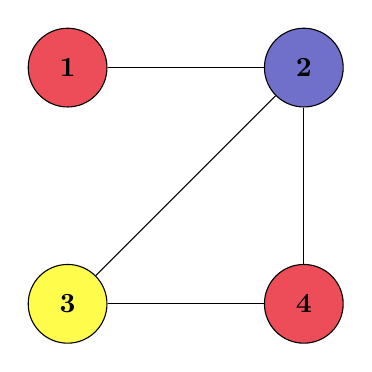
\begin{tikzpicture}[x=1.5cm, y=1.5cm]
  % 設定
  \tikzset{node/.style={circle,draw=black,minimum size=1cm}}
 
  % 色
  \definecolor{red}{RGB}{230,0,18}
  \definecolor{blue}{RGB}{51,51,179}
  \definecolor{yellow}{RGB}{255,251,0}
 
  % 補助線
  % \draw [help lines,blue] (0,0) grid (20,6);
 
  % node %
  \node[node, fill=red!70] at (-1,1) (node1) {\textbf{1}};
  \node[node, fill=blue!70] at (1,1) (node2) {\textbf{2}};
  \node[node, fill=yellow!70] at (-1,-1) (node3) {\textbf{3}};
  \node[node, fill=red!70] at (1,-1) (node4) {\textbf{4}};
 
  \foreach \u / \v in {node1/node2, node2/node3, node2/node4, node3/node4}
  \draw (\u) -- (\v);
\end{tikzpicture}
}
    \end{tabular}
  \end{exampleblock}
  \pause
  \begin{block}{$k$彩色遷移問題}
    \begin{itemize}
    \item \structure{\bf 入力}:
      色数$k$のグラフ点彩色問題と,スタート状態とゴール状態
      を表す2つの実行可能解
    \item \structure{遷移制約}: 1回の遷移で色が変化する頂点はただ1つのみ
    \item \structure{目的}:
      スタート状態からゴール状態への到達可能性を判定
    \end{itemize}
  \end{block}
  \begin{itemize}
  \item 代表的な組合せ遷移問題の一つである.
  \item 一般に$k \geq 4$で PSPACE 完全であることが知られている.
  \end{itemize}

\end{frame}
%%%%%%%%%%%%%%%%%%%%%%%%%%%%%%%%%%%%%%%%%%%%%%%%%%%%%%%%%%%%%%%%%
\begin{frame}%[shrink]
  \frametitle{$k=4$彩色遷移問題の例}
  \begin{center}
  \tabcolsep = 3mm
  \renewcommand{\arraystretch}{1.2}
  \begin{tabular}[t]{ccc}
    スタート状態($t=0$) && \uncover<2>{$t=1$} \\
    \scalebox{0.5}{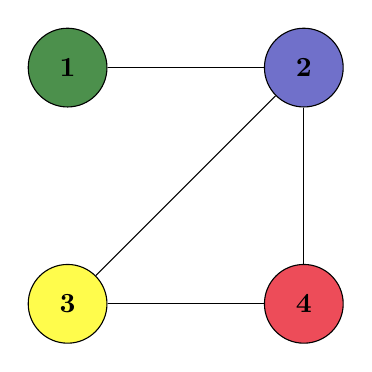
\begin{tikzpicture}[x=1.5cm, y=1.5cm]
  % 設定
  \tikzset{node/.style={circle,draw=black,minimum size=1cm}}
 
  %色
  \definecolor{red}{RGB}{230,0,18}
  \definecolor{blue}{RGB}{51,51,179}
  \definecolor{yellow}{RGB}{255,251,0}
  \definecolor{green}{RGB}{0,96,0}
 
  % 補助線
  % \draw [help lines,blue] (0,0) grid (20,6);
 
  % node %
  \node[node, fill=green!70] at (-1,1) (node1) {\textbf{1}};
  \node[node, fill=blue!70] at (1,1) (node2) {\textbf{2}};
  \node[node, fill=yellow!70] at (-1,-1) (node3) {\textbf{3}};
  \node[node, fill=red!70] at (1,-1) (node4) {\textbf{4}};
 
  \foreach \u / \v in {node1/node2, node2/node3, node2/node4, node3/node4}
  \draw (\u) -- (\v);
\end{tikzpicture}
} &
    \uncover<2>{\rz{\Large$\Rightarrow$}} &
    \uncover<2>{\scalebox{0.5}{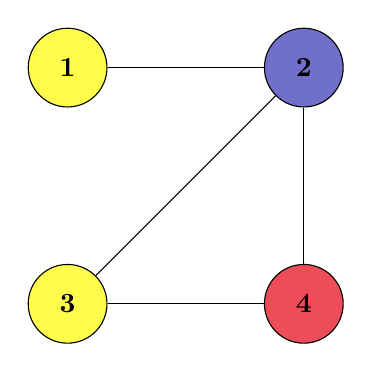
\begin{tikzpicture}[x=1.5cm, y=1.5cm]
  % 設定
  \tikzset{node/.style={circle,draw=black,minimum size=1cm}}
 
  %色
  \definecolor{red}{RGB}{230,0,18}
  \definecolor{blue}{RGB}{51,51,179}
  \definecolor{yellow}{RGB}{255,251,0}
  \definecolor{green}{RGB}{0,96,0}
 
  % 補助線
  % \draw [help lines,blue] (0,0) grid (20,6);
 
  % node %
  \node[node, fill=yellow!70] at (-1,1) (node1) {\textbf{1}};
  \node[node, fill=blue!70] at (1,1) (node2) {\textbf{2}};
  \node[node, fill=yellow!70] at (-1,-1) (node3) {\textbf{3}};
  \node[node, fill=red!70] at (1,-1) (node4) {\textbf{4}};
 
  \foreach \u / \v in {node1/node2, node2/node3, node2/node4, node3/node4}
  \draw (\u) -- (\v);
\end{tikzpicture}
}}\\
    && \uncover<2>{\Large $\Downarrow$} \\
    \scalebox{0.5}{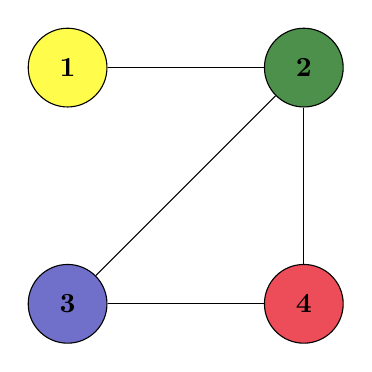
\begin{tikzpicture}[x=1.5cm, y=1.5cm]
  % 設定
  \tikzset{node/.style={circle,draw=black,minimum size=1cm}}
 
  %色
  \definecolor{red}{RGB}{230,0,18}
  \definecolor{blue}{RGB}{51,51,179}
  \definecolor{yellow}{RGB}{255,251,0}
  \definecolor{green}{RGB}{0,96,0}
 
  % 補助線
  % \draw [help lines,blue] (0,0) grid (20,6);
 
  % node %
  \node[node, fill=yellow!70] at (-1,1) (node1) {\textbf{1}};
  \node[node, fill=green!70] at (1,1) (node2) {\textbf{2}};
  \node[node, fill=blue!70] at (-1,-1) (node3) {\textbf{3}};
  \node[node, fill=red!70] at (1,-1) (node4) {\textbf{4}};
 
  \foreach \u / \v in {node1/node2, node2/node3, node2/node4, node3/node4}
  \draw (\u) -- (\v);
\end{tikzpicture}
} &
    \uncover<2>{\rz{\Large$\Leftarrow$}} &
    \uncover<2>{\scalebox{0.5}{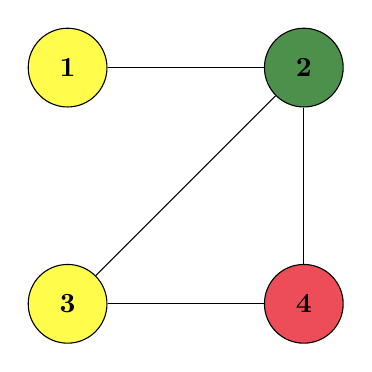
\begin{tikzpicture}[x=1.5cm, y=1.5cm]
  % 設定
  \tikzset{node/.style={circle,draw=black,minimum size=1cm}}
 
  %色
  \definecolor{red}{RGB}{230,0,18}
  \definecolor{blue}{RGB}{51,51,179}
  \definecolor{yellow}{RGB}{255,251,0}
  \definecolor{green}{RGB}{0,96,0}
 
  % 補助線
  % \draw [help lines,blue] (0,0) grid (20,6);
 
  % node %
  \node[node, fill=yellow!70] at (-1,1) (node1) {\textbf{1}};
  \node[node, fill=green!70] at (1,1) (node2) {\textbf{2}};
  \node[node, fill=yellow!70] at (-1,-1) (node3) {\textbf{3}};
  \node[node, fill=red!70] at (1,-1) (node4) {\textbf{4}};
 
  \foreach \u / \v in {node1/node2, node2/node3, node2/node4, node3/node4}
  \draw (\u) -- (\v);
\end{tikzpicture}
}}\\
    ゴール状態\uncover<2>{($t=3$)} && \uncover<2>{$t=2$}
  \end{tabular}
  \end{center}

  \uncover<2>{
  \begin{itemize}
  \item スタート状態からゴール状態へ3ステップで到達可能である.
  \item 各ステップ$t$において,グラフ点彩色問題の制約を満たす.
  \item 1回の遷移において,色が変化する頂点はただ1つのみである.
  \end{itemize}
  }
\end{frame}
%%%%%%%%%%%%%%%%%%%%%%%%%%%%%%%%%%%%%%%%%%%%%%%%%%%%%%%%%%%%%%%%%
\begin{frame}
  \frametitle{解集合プログラミング {\large(Answer Set Programming; ASP)}}
  \begin{itemize}
  \item \structure{ASP 言語}は,一階論理に基づく知識表現言語の一種.
  \item \structure{ASP システム}は,論理プログラムから
    安定モデル意味論~{\scriptsize[Gelfond and Lifschitz, '88]}
    に基づく解集合を計算するシステム.
  \item 近年,SAT 技術を応用した高速 ASP システムが開発され,
    システム生物学,プランニング,モデル検査など様々な分野への実用的応
    用が急速に拡大している.
  \end{itemize}

  \begin{alertblock}{組合せ遷移問題に対してASPを用いる利点}
    \begin{itemize}
    \item ASPの高い表現力により,様々な組合せ問題を簡潔に記述できる.
      \begin{itemize}
      \item \alert{\bf 遷移問題への拡張も容易}.
      \end{itemize}
    \item インクリメンタルASP解法により,ステップ長を増やしながら,
      遷移問題の\alert{\bf 到達可能性を効率的に検査}できる.
      \begin{itemize}
      \item ASP システムを複数回起動するオーバーヘッドを回避.
      \item 同様の探索失敗を避けるために獲得した学習節を再利用.
      \end{itemize}
    \item 探索ヒューリスティックスを簡単にカスタマイズできる.
    % \item ASP Modulo Theories 技術により,様々な背景理論ソルバーと連携が可能である.
    \end{itemize}
  \end{alertblock}
\end{frame}
%%%%%%%%%%%%%%%%%%%%%%%%%%%%%%%%%%%%%%%%%%%%%%%%%%%%%%%%%%%%%%%%% 
\begin{frame}
  \frametitle{研究目的}
  \begin{alertblock}{研究目的}
    ASP 技術を活用し,組合せ遷移問題を効率よく解くソルバーを実現する.
  \end{alertblock}
  \begin{itemize}
  \item 方針: プランニングや有界モデル検査のための技法を応用
  \end{itemize}
  \begin{block}{研究内容}
    \begin{enumerate}
    \item \structure{有界組合せ遷移(Bounded Combinatorial Reconfiguration)の提案}
      \begin{itemize}
      \item ASP 技術を用いた組合せ遷移問題の解法
      \end{itemize}
    \item \structure{ASP 技術を用いた組合せ遷移ソルバーの実装方式の提案}
      \begin{itemize}
      \item 基本アルゴリズム
      \item インクリメンタルASP解法を用いた改良アルゴリズム
      \end{itemize}
    \item \structure{$k$彩色遷移問題を解く ASP 符号化の考案}
      \begin{itemize}
      \item \textsf{changed}符号化
      \item \textsf{unchanged}符号化 (本発表では省略)
      \end{itemize}
    \item \structure{$k$彩色遷移問題のベンチマーク問題を独自に生成}
    \item \structure{$k$彩色遷移問題を用いた有界組合せ遷移の評価実験}
    \end{enumerate}
  \end{block}
\end{frame}
%%%%%%%%%%%%%%%%%%%%%%%%%%%%%%%%%%%%%%%%%%%%%%%%%%%%%%%%%%%%%%%%% 
\begin{frame}
  \frametitle{有界組合せ遷移の基本アイデア (提案)}
  \begin{itemize}
  \item 基の組合せ問題の変数集合
    $\bm{x} = \{x_1,x_2,\ldots,x_n\}$
    に対して,ステップ$t\geq 0$での各変数の値を表す変数集合を
    $\bm{x}^{t} = \{x_1^t,x_2^t,\ldots,x_n^t\}$を導入.
  \item スタート状態から$\ell$ステップ遷移した後の各変数の値
    $\bm{x}^{\ell}$が,ゴール状態を満足するかを判定するため,
    論理式$\varphi_{\ell}$を構成する.
  \end{itemize}
  \begin{block}{}\centering\vskip-1em
  \begin{align*}
  \varphi_{\ell} &= S(\bm{x}^0)  & S: \textrm{スタート状態を表す論理式} \\
  &\land \bigwedge_{t=0}^{\ell} C(\bm{x}^t) & C: \textrm{基の組合せ問題の制約を表す論理式} \\
  &\land \bigwedge_{t=1}^{\ell} T(\bm{x}^{t-1},\bm{x}^{t}) & T: \textrm{遷移制約を表す論理式} \\
  &\land G(\bm{x}^\ell)  & G: \textrm{ゴール状態を表す論理式}
  \end{align*}
  \end{block}
  \begin{itemize}
  \item \bm{$\varphi_{\ell}$}が充足可能の場合,
    ステップ長$\ell$の到達可能な遷移系列が存在する
    ことを意味する.
  \end{itemize}
\end{frame}
%%%%%%%%%%%%%%%%%%%%%%%%%%%%%%%%%%%%%%%%%%%%%%%%%%%%%%%%%%%%%%%%% 
\begin{frame}%[shrink]
  \frametitle{有界組合せ遷移 (提案)} 
  \begin{alertblock}{有界組合せ遷移}\centering
    組合せ遷移問題に対して,制限された長さ (すなわち,有界)の
    遷移系列
    \[
    \varphi_{\ell} = S(\bm{x}^0)  
    \land \bigwedge_{t=0}^{\ell} C(\bm{x}^t) 
    \land \bigwedge_{t=1}^{\ell} T(\bm{x}^{t-1},\bm{x}^{t}) 
    \land G(\bm{x}^\ell)  
    \]
    を論理プログラムとして表現し,
    ASP システムを用いて実行することにより,到達可能性の検査を行う手法
  \end{alertblock}
  \begin{itemize}
  \item $\varphi_{\ell}$が\structure{充足可能}の場合,
    ステップ長$\ell$の\structure{到達可能}な遷移系列が存在.
  \item \structure{充足不能}の場合,ステップ長$\ell$では\structure{到達不能}.
    この場合,$\ell$を増加させた論理プログラムを再構成し,
    繰り返し ASP システムを実行.
  \item この手法は,到達不能の証明は行わない不完全な手続きである.
    \begin{itemize}
      \item ただし,検査すべき遷移系列のステップ長に上限~\footnotemark[2]
        が存在する場合には,完全な手続きとなる.
    \end{itemize}
  \end{itemize}
  \footnotetext[2]{例えば,任意の2つの実行可能解の最短経路のうちの最大長(問題の直径)}
\end{frame}
%%%%%%%%%%%%%%%%%%%%%%%%%%%%%%%%%%%%%%%%%%%%%%%%%%%%%%%%%%%%%%%%%%%
\begin{frame}{ASP 技術を用いた組合せ遷移ソルバーの実装}

\begin{alertblock}{}\centering
開発した組合せ遷移ソルバーの構成図は以下の通りである.
\end{alertblock}
\vfill
\begin{center}
\setlength{\unitlength}{1.0pt}
\scriptsize\tiny
\thicklines
%    \thicklines
  \setlength{\unitlength}{1.28pt}
  \small
  \begin{picture}(280,57)(4,-10)
    \put(  0, 20){\dashbox(50,24){\shortstack{根付き全域森\\問題}}}
    \put( 60, 20){\framebox(50,24){変換器}}
    \put(120, 20){\dashbox(50,24){\shortstack{ASPファクト}}}
    \put(120,-10){\alert{\bf\dashbox(50,24){\scriptsize{\shortstack{ASP符号化\\(論理プログラム)}}}}}
    \put(180, 20){\framebox(50,24){ASPシステム}}
    \put(240, 20){\dashbox(50,24){\shortstack{根付き全域森\\問題の解}}}
    \put( 50, 32){\vector(1,0){10}}
    \put(110, 32){\vector(1,0){10}}
    \put(170, 32){\vector(1,0){10}}
    \put(230, 32){\vector(1,0){10}}
    \put(170, +2){\line(1,0){4}}
    \put(174, +2){\line(0,1){30}}
  \end{picture}  

\begin{picture}(280,57)(4,-10)
  \put(  0, 20){\dashbox(50,24){\shortstack{組合せ遷移問題\\のインスタンス}}}
  \put( 60, 20){\framebox(50,24){変換器}}
  \put(120, 20){\dashbox(50,24){\shortstack{ASPファクト}}}
  \put(120,-10){\dashbox(50,24){\shortstack{論理プログラム\\(ASP符号化)}}}
  \put(180,-10){\alert{\framebox(50,54){}}}
  \put(185, 27){\framebox(40,12){ASP システム}}
  \put(185, -5){\framebox(40,18){\shortstack{有界組合せ遷移\\アルゴリズム}}}
  \put(240, 20){\dashbox(50,24){\shortstack{組合せ遷移問題\\の解}}}
  \put( 50, 32){\vector(1,0){10}}
  \put(110, 32){\vector(1,0){10}}
  \put(170, 32){\vector(1,0){10}}
  \put(230, 32){\vector(1,0){10}}
  \put(170, +2){\line(1,0){4}}
  \put(174, +2){\line(0,1){30}}
  \put(195, 13){\vector(0,1){14}}
  \put(215, 27){\vector(0,-1){14}}
  \put(188, 50){\alert{\bf 提案ソルバー}}
\end{picture}  
\end{center}
  
\begin{enumerate}
\item 問題インスタンスを ASP のファクト形式に変換する.
\item ASP ファクトと組合せ遷移問題を解く
  論理プログラム(ASP符号化)を入力として,
  \alert{\bf 提案ソルバー}を用いて解集合を計算する.
\item 解集合を解釈して,組合せ遷移問題の解を得る.
\end{enumerate}
\end{frame}
%%%%%%%%%%%%%%%%%%%%%%%%%%%%%%%%%%%%%%%%%%%%%%%%%%%%%%%%%%%%%%%%%%%
\begin{frame}[shrink]{有界組合せ遷移アルゴリズム}

\begin{alertblock}{}\centering
有界組合せ遷移のためのアルゴリズムを2種類考案した.
\end{alertblock}

\begin{center}
\setlength{\unitlength}{1.0pt}
\scriptsize\tiny
\thicklines
%    \thicklines
  \setlength{\unitlength}{1.28pt}
  \small
  \begin{picture}(280,57)(4,-10)
    \put(  0, 20){\dashbox(50,24){\shortstack{根付き全域森\\問題}}}
    \put( 60, 20){\framebox(50,24){変換器}}
    \put(120, 20){\dashbox(50,24){\shortstack{ASPファクト}}}
    \put(120,-10){\alert{\bf\dashbox(50,24){\scriptsize{\shortstack{ASP符号化\\(論理プログラム)}}}}}
    \put(180, 20){\framebox(50,24){ASPシステム}}
    \put(240, 20){\dashbox(50,24){\shortstack{根付き全域森\\問題の解}}}
    \put( 50, 32){\vector(1,0){10}}
    \put(110, 32){\vector(1,0){10}}
    \put(170, 32){\vector(1,0){10}}
    \put(230, 32){\vector(1,0){10}}
    \put(170, +2){\line(1,0){4}}
    \put(174, +2){\line(0,1){30}}
  \end{picture}  

\begin{picture}(280,57)(4,-10)
  \put(  0, 20){\dashbox(50,24){\shortstack{組合せ遷移問題\\のインスタンス}}}
  \put( 60, 20){\framebox(50,24){変換器}}
  \put(120, 20){\dashbox(50,24){\shortstack{ASPファクト}}}
  \put(120,-10){\dashbox(50,24){\shortstack{論理プログラム\\(ASP符号化)}}}
  \put(180,-10){\framebox(50,54){}}
  \put(185, 27){\framebox(40,12){ASP システム}}
  \put(185, -5){\alert{\bf\framebox(40,18){\shortstack{有界組合せ遷移\\アルゴリズム}}}}
  \put(240, 20){\dashbox(50,24){\shortstack{組合せ遷移問題\\の解}}}
  \put( 50, 32){\vector(1,0){10}}
  \put(110, 32){\vector(1,0){10}}
  \put(170, 32){\vector(1,0){10}}
  \put(230, 32){\vector(1,0){10}}
  \put(170, +2){\line(1,0){4}}
  \put(174, +2){\line(0,1){30}}
  \put(195, 13){\vector(0,1){14}}
  \put(215, 27){\vector(0,-1){14}}
  \put(188, 50){提案ソルバー}
\end{picture}  
\end{center}
  
\begin{enumerate}
\item \structure{基本アルゴリズム}
  \begin{itemize}
  \item ステップ長$\ell$を増加させながら,
    $\varphi_{\ell}$を繰り返し構成し解く.
  \item 長所: 実装が単純である.
  \item 短所: 学習節が再利用できない.
  \item 短所: ASPシステムを毎回起動するオーバーヘッドが大きい.
  \end{itemize}
\item \structure{インクリメンタルASP解法を用いた改良アルゴリズム}
  \begin{itemize}
  \item $S(\bm{x}^{0})$, $C(\bm{x}^{t})$,
    $T(\bm{x}^{t-1},\bm{x}^{t})$, $G(\bm{x}^{t})$
    を動的に追加・削除しながら,$\varphi_{\ell}$をインクリメンタルに構成し解く.
  \item 長所: 学習節の再利用が可能.ASPシステムの起動は1回のみ.
  \item 短所: 現状では,デバックしにくい.
  \end{itemize}
\end{enumerate}
\end{frame}
%%%%%%%%%%%%%%%%%%%%%%%%%%%%%%%%%%%%%%%%%%%%%%%%%%%%%%%%%%%%%%%%%%%
\begin{frame}
  \frametitle{基本アルゴリズム}

  \[
    \varphi_{\ell} = S(\bm{x}^0)  
    \land \bigwedge_{t=0}^{\ell} C(\bm{x}^t) 
    \land \bigwedge_{t=1}^{\ell} T(\bm{x}^{t-1},\bm{x}^{t}) 
    \land G(\bm{x}^\ell)  
  \]

\begin{block}{基本アルゴリズムの手続き}
\begin{enumerate}
\item ステップ長$\ell$を$\ell=0$とする.
%\item \label{BoCoRe:base:solver:2}
%  $\varphi_\ell$を論理プログラムとして記述し,
%  ファクト形式の問題インスタンスとともに,
%  ASP システムに入力として与える.
\item \label{BoCoRe:base:solver:2}
  $\varphi_\ell$を論理プログラムとして記述した
  $\enc{\varphi_\ell}$と
  ファクト形式の問題インスタンスとともに,
  ASP システムに入力として与える.
\item ASP システムの出力結果が充足可能であれば終了する.
  充足不能であれば$\ell$の値を1増加させ,
  (\ref{BoCoRe:base:solver:2})に戻り手続きを繰り返す.
  \begin{itemize}
  \item ただし,$\ell$が問題の直径を超えたところで繰り返しを停止できる.
  \end{itemize}
\end{enumerate}
\end{block}

\begin{itemize}
\item この手続きは,与えられた組合せ遷移問題に対して,
 到達可能な\structure{最短の遷移系列}を探索する.
\end{itemize}
\end{frame}
%%%%%%%%%%%%%%%%%%%%%%%%%%%%%%%%%%%%%%%%%%%%%%%%%%%%%%%%%%%%%%%%%%% 
\begin{frame}\frametitle{基本アルゴリズムの問題点}

  \begin{block}{}
    \vskip -1em
    \begin{align*}
    \varphi_{\ell-1} &= S(\bm{x}^0)
    \land \bigwedge_{t=0}^{\ell-1} C(\bm{x}^t) 
    \land \bigwedge_{t=1}^{\ell-1} T(\bm{x}^{t-1},\bm{x}^{t})
    \land G(\bm{x}^{\ell-1})\\
    \varphi_{\ell} &= S(\bm{x}^0)
    \land \bigwedge_{t=0}^{\ell} C(\bm{x}^t) 
    \land \bigwedge_{t=1}^{\ell} T(\bm{x}^{t-1},\bm{x}^{t})
    \land G(\bm{x}^\ell)
  \end{align*}
  \end{block}
  
  \begin{itemize}
  \item $\varphi_{\ell-1}$と$\varphi_{\ell}$は共通部分が多いため,
    \structure{同じ探索空間を繰り返し調べる}ことになる.
  \item 各$\varphi_\ell$に対して,毎回 ASP システムを起動するため,
    \structure{学習節の再利用ができない}.
  \item また,ステップ長$\ell$が大きくなった場合,
    毎回 \structure{ASP システムを起動するオーバヘッド}も無視できない.
  \end{itemize}

  \begin{alertblock}{改善のためのアイデア}\centering
    $\varphi_{\ell}$は,$\varphi_{\ell-1}$に
    $C(\bm{x}^{\ell})$と$T(\bm{x}^{\ell-1},\bm{x}^{\ell})$と
    $G(\bm{x}^{\ell})$を追加し,$G(\bm{x}^{\ell-1})$を削除することで,
    インクリメンタルに構成できる.    
  \end{alertblock}
\end{frame}
%%%%%%%%%%%%%%%%%%%%%%%%%%%%%%%%%%%%%%%%%%%%%%%%%%%%%%%%%%%%%%%%%%%
\begin{frame}\frametitle{改良アルゴリズム}

  \begin{block}{改良アルゴリズムの手続き}
    \begin{enumerate}
    \item ASP システムを起動する.
    \item ステップ$t$を$t=0$,論理プログラム
      $\Psi$を$\Psi = \emptyset$とする.
    \item $t>0$であれば,
      $\Psi = \Psi - \enc{G(\bm{x}^{t-1})}$
      \label{improved_solver:loop}
    \item $t=0$であれば,
      $\Psi = \Psi\ \cup\ \enc{\textrm{問題インスタンス}} \cup\ \enc{S(\bm{x}^0)}$
    \item $\Psi = \Psi \ \cup \ \enc{C(\bm{x}^{t})} \ \cup \ 
      \enc{T(\bm{x}^{t-1},\bm{x}^{t})} \ \cup \ \enc{G(\bm{x}^{t})}$
    \item $\Psi$を実行する.
    \item 実行結果が充足可能であれば終了する.
      充足不能であれば$t$の値を1増加させ,
      (\ref{improved_solver:loop})に戻り手続きを繰り返す.
      \begin{itemize}
      \item ただし,$t$がステップ長の上限値を超えたところで
        繰り返しを停止できる.
      \end{itemize} \label{improved_solver:end}
    \end{enumerate}
  \end{block}

  \begin{itemize}
  \item 改良アルゴリズムは,ASP システム{\clingo}の python インターフェー
    スを用いて簡潔に実装できる(37行程度).
  \end{itemize}

\end{frame}
%%%%%%%%%%%%%%%%%%%%%%%%%%%%%%%%%%%%%%%%%%%%%%%%%%%%%%%%%%%%%%%%%%%
\begin{frame}
  \frametitle{提案ソルバーを用いた$k$彩色遷移問題の解法}

\begin{alertblock}{}\centering
  $k$彩色遷移問題を例にとって,提案ソルバーを用いた解法を示す.
\end{alertblock}
\vfill
\begin{center}
\setlength{\unitlength}{1.0pt}
\scriptsize\tiny
\thicklines
%    \thicklines
  \setlength{\unitlength}{1.28pt}
  \small
  \begin{picture}(280,57)(4,-10)
    \put(  0, 20){\dashbox(50,24){\shortstack{根付き全域森\\問題}}}
    \put( 60, 20){\framebox(50,24){変換器}}
    \put(120, 20){\dashbox(50,24){\shortstack{ASPファクト}}}
    \put(120,-10){\alert{\bf\dashbox(50,24){\scriptsize{\shortstack{ASP符号化\\(論理プログラム)}}}}}
    \put(180, 20){\framebox(50,24){ASPシステム}}
    \put(240, 20){\dashbox(50,24){\shortstack{根付き全域森\\問題の解}}}
    \put( 50, 32){\vector(1,0){10}}
    \put(110, 32){\vector(1,0){10}}
    \put(170, 32){\vector(1,0){10}}
    \put(230, 32){\vector(1,0){10}}
    \put(170, +2){\line(1,0){4}}
    \put(174, +2){\line(0,1){30}}
  \end{picture}  

\begin{picture}(280,57)(4,-10)
  \put(  0, 20){\dashbox(50,24){\shortstack{$k$彩色遷移問題\\のインスタンス}}}
  \put( 60, 20){\framebox(50,24){変換器}}
  \put(120, 20){\alert{\bf \dashbox(50,24){\shortstack{ASPファクト}}}}
  \put(120,-10){\alert{\bf \dashbox(50,24){\shortstack{論理プログラム\\(ASP符号化)}}}}
  \put(180,-10){\framebox(50,54){}}
  \put(185, 27){\framebox(40,12){ASP システム}}
  \put(185, -5){\framebox(40,18){\shortstack{有界組合せ遷移\\アルゴリズム}}}
  \put(240, 20){\alert{\bf \dashbox(50,24){\shortstack{$k$彩色遷移問題\\の解}}}}
  \put( 50, 32){\vector(1,0){10}}
  \put(110, 32){\vector(1,0){10}}
  \put(170, 32){\vector(1,0){10}}
  \put(230, 32){\vector(1,0){10}}
  \put(170, +2){\line(1,0){4}}
  \put(174, +2){\line(0,1){30}}
  \put(195, 13){\vector(0,1){14}}
  \put(215, 27){\vector(0,-1){14}}
  \put(188, 50){提案ソルバー}
\end{picture}  
\end{center}
\begin{enumerate}
\item $k$彩色遷移問題のASPファクト形式
\item $k$彩色遷移問題を解く ASP 符号化
  \begin{tabular}[t]{lcl}
    \structure{\textsf{changed} 符号化}   & : & 色が変化した頂点数をカウント\\
    \structure{\textsf{unchanged} 符号化} & : & 色が変化しなかった頂点数をカウント
  \end{tabular}
\item 提案ソルバーの実行例
\end{enumerate}
\end{frame}
%%%%%%%%%%%%%%%%%%%%%%%%%%%%%%%%%%%%%%%%%%%%%%%%%%%%%%%%%%%%%%%%%%%
\begin{frame}
  \frametitle{$k$彩色遷移問題のファクト形式}

\begin{center}
  \tabcolsep = 3mm
  \renewcommand{\arraystretch}{1.2}
  \begin{tabular}[t]{ccc}
    スタート状態 && ゴール状態 \\
    \scalebox{0.5}{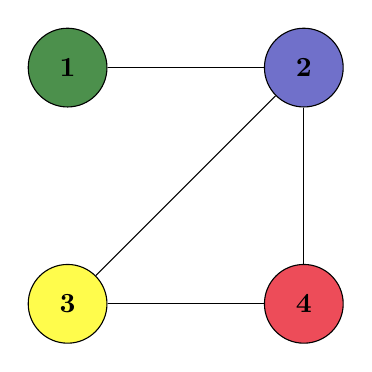
\begin{tikzpicture}[x=1.5cm, y=1.5cm]
  % 設定
  \tikzset{node/.style={circle,draw=black,minimum size=1cm}}
 
  %色
  \definecolor{red}{RGB}{230,0,18}
  \definecolor{blue}{RGB}{51,51,179}
  \definecolor{yellow}{RGB}{255,251,0}
  \definecolor{green}{RGB}{0,96,0}
 
  % 補助線
  % \draw [help lines,blue] (0,0) grid (20,6);
 
  % node %
  \node[node, fill=green!70] at (-1,1) (node1) {\textbf{1}};
  \node[node, fill=blue!70] at (1,1) (node2) {\textbf{2}};
  \node[node, fill=yellow!70] at (-1,-1) (node3) {\textbf{3}};
  \node[node, fill=red!70] at (1,-1) (node4) {\textbf{4}};
 
  \foreach \u / \v in {node1/node2, node2/node3, node2/node4, node3/node4}
  \draw (\u) -- (\v);
\end{tikzpicture}
} &&
    \scalebox{0.5}{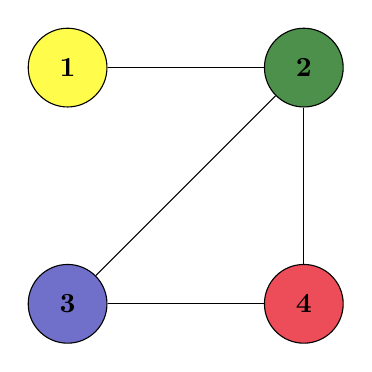
\begin{tikzpicture}[x=1.5cm, y=1.5cm]
  % 設定
  \tikzset{node/.style={circle,draw=black,minimum size=1cm}}
 
  %色
  \definecolor{red}{RGB}{230,0,18}
  \definecolor{blue}{RGB}{51,51,179}
  \definecolor{yellow}{RGB}{255,251,0}
  \definecolor{green}{RGB}{0,96,0}
 
  % 補助線
  % \draw [help lines,blue] (0,0) grid (20,6);
 
  % node %
  \node[node, fill=yellow!70] at (-1,1) (node1) {\textbf{1}};
  \node[node, fill=green!70] at (1,1) (node2) {\textbf{2}};
  \node[node, fill=blue!70] at (-1,-1) (node3) {\textbf{3}};
  \node[node, fill=red!70] at (1,-1) (node4) {\textbf{4}};
 
  \foreach \u / \v in {node1/node2, node2/node3, node2/node4, node3/node4}
  \draw (\u) -- (\v);
\end{tikzpicture}
} 
  \end{tabular}
\end{center}
\vfill
\begin{exampleblock}{$4$彩色遷移問題の例 (\code{graph_reconfig.lp})}
\lstinputlisting[frame=none,numbers=none,basicstyle=\ttfamily\footnotesize]{code/graph_reconfig.lp} 
\end{exampleblock}    

\begin{itemize}
\item アトム\code{node/1}は頂点,\code{edge/2}は辺を表す.
\item アトム\code{start(X,C)} は,スタート状態で頂点\code{X}が色\code{C}で
  塗られることを意味する.\code{goal(X,C)}はゴール状態を表す.
%  \item 色1は赤,色2は青,色3は黄,色4は緑に対応している.
\end{itemize}
\end{frame}
%%%%%%%%%%%%%%%%%%%%%%%%%%%%%%%%%%%%%%%%%%%%%%%%%%%%%%%%%%%%%%%%%%%
\begin{frame}[shrink]
  \frametitle{$k$彩色遷移問題を解く\code{changed} 符号化 {\small(基本ソルバー用)}}

\begin{columns}[t]
\begin{column}{0.95\linewidth}
\begin{exampleblock}{\code{changed.lp}}
\lstinputlisting[frame=none,numbers=left,basicstyle=\ttfamily\scriptsize]{code/gcrp_cc_changed.lp} 
\end{exampleblock}    
\end{column}
\end{columns}

\bigskip
\begin{itemize}
  \item 8個のルールで簡潔に記述可能である.
\end{itemize}

% \only<2>{
%   \begin{itemize}
%   \item 1行目: 定数\code{c} は色数,定数\code{length} はステップ長を表す.
%     これらは,実行時にASPシステムのオプションから与えられる.
%   \item アトム\code{col/1}は色,アトム\code{t/1} はステップを表す.
%   \item 3行目: スタート状態の制約$S(\bm{x}^0)$を表す.
%   \end{itemize}
% }
% \only<3>{
% \begin{itemize}
%   \item 5--7行目: グラフ点彩色問題の制約$C(\bm{x}^{t})$を表す.
%   \item アトム\code{color(X,C,T)}は,ステップ\code{T}で頂点\code{X}が色
%     \code{C}で塗られることを意味する.
%   \item 5行目: 各ステップ\code{T},各頂点\code{X}に対して,
%     \code{X}がただ1つの色で塗られることを個数制約を用いて表している.
%   \item 6--7行目: 各ステップ\code{T},各辺\code{edge(X,Y)}に対して,
%     隣接する頂点\code{X}と\code{Y}が同じ色で塗られないことを表す.
% \end{itemize}
% }
% \only<4>{
%   \begin{itemize}
%   \item 9--10行目: 遷移制約$T(\bm{x}^{t-1},\bm{x}^{t})$を表す.
%   \item アトム\code{changed(X,T)}は,ステップ\code{T-1}とステップ\code{T}の間
%     で,頂点\code{X}の色が変化したことを意味する.
%   \item 10行目: 各ステップ\code{T}において,色が変化する頂点はただ1つ
%     であることを表す.
%   \item 12行目: ゴール状態の制約$G(\bm{x}^{\ell})$を表す.
%   \end{itemize}
% }
\end{frame}
%%%%%%%%%%%%%%%%%%%%%%%%%%%%%%%%%%%%%%%%%%%%%%%%%%%%%%%%%%%%%%%%%%%
\begin{frame}[shrink]
  \frametitle{$k$彩色遷移問題を解く \code{changed} 符号化 {\small(改良アルゴリズム用)}}

\begin{columns}[t]
\begin{column}{0.9\linewidth}
\begin{exampleblock}{\code{changed} 符号化 (\code{changed_inc.lp})}
\lstinputlisting[frame=none,numbers=left,basicstyle=\ttfamily\scriptsize]{code/gcrp_cc_changed_inc.lp} 
\end{exampleblock}    
\end{column}
\end{columns}

\begin{itemize}
\item 3つのサブプログラム
  \code{base}, \code{step(t)}, \code{check(t)}
  から構成される.
% \item 記号\code{t} は,ステップを表す.
  \begin{itemize}
  \item \code{base} : スタート状態の制約$S(\bm{x}^0)$
  \item \code{step(t)} : グラフ点彩色問題の制約$C(\bm{x}^{t})$と
    遷移制約$T(\bm{x}^{t-1},\bm{x}^{t})$
  \item \code{check(t)} : ゴール状態の制約$G(\bm{x}^{t})$
  \end{itemize}
\end{itemize}
\end{frame}
%%%%%%%%%%%%%%%%%%%%%%%%%%%%%%%%%%%%%%%%%%%%%%%%%%%%%%%%%%%%%%%%%%%
\begin{frame}[shrink]
  \frametitle{提案ソルバーの実行例{\small (基本アルゴリズム)}}

%\begin{columns}[t]
%\begin{column}{0.9\linewidth}
\begin{exampleblock}{}
\lstinputlisting[frame=none,numbers=none,basicstyle=\ttfamily\tiny]{code/graph_reconfig.log} 
\end{exampleblock}    
%\end{column}
%\end{columns}
  
\end{frame}
%%%%%%%%%%%%%%%%%%%%%%%%%%%%%%%%%%%%%%%%%%%%%%%%%%%%%%%%%%%%%%%%%%%
\begin{frame}%[shrink]
  \frametitle{提案ソルバーの実行例{\small (改良アルゴリズム)}}

  \begin{exampleblock}{}
    \lstinputlisting[frame=none,numbers=none,basicstyle=\ttfamily\scriptsize]{code/graph_reconfig_inc.log} 
  \end{exampleblock}
  \begin{itemize}
  \item \code{core.lp}は,改良アルゴリズムを実装したpythonプログラム
  \item \code{color(X,C,T)}はステップ\code{T} で頂点\code{X} が色\code{C}
    で塗られることを意味
  \end{itemize}
\end{frame}
%%%%%%%%%%%%%%%%%%%%%%%%%%%%%%%%%%%%%%%%%%%%%%%%%%%%%%%%%%%%%%%%%%%
\begin{frame}
  \frametitle{得られた遷移系列}

  \begin{center}
  \tabcolsep = 3mm
  \renewcommand{\arraystretch}{1.2}
  \begin{tabular}[t]{ccc}
    スタート状態($t=0$) && $t=1$ \\
    \scalebox{0.5}{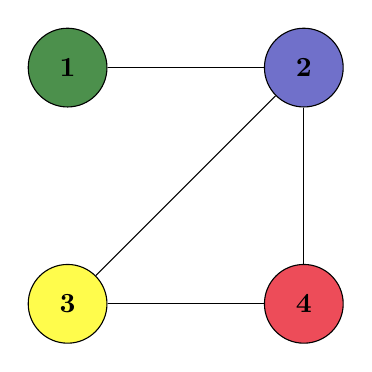
\begin{tikzpicture}[x=1.5cm, y=1.5cm]
  % 設定
  \tikzset{node/.style={circle,draw=black,minimum size=1cm}}
 
  %色
  \definecolor{red}{RGB}{230,0,18}
  \definecolor{blue}{RGB}{51,51,179}
  \definecolor{yellow}{RGB}{255,251,0}
  \definecolor{green}{RGB}{0,96,0}
 
  % 補助線
  % \draw [help lines,blue] (0,0) grid (20,6);
 
  % node %
  \node[node, fill=green!70] at (-1,1) (node1) {\textbf{1}};
  \node[node, fill=blue!70] at (1,1) (node2) {\textbf{2}};
  \node[node, fill=yellow!70] at (-1,-1) (node3) {\textbf{3}};
  \node[node, fill=red!70] at (1,-1) (node4) {\textbf{4}};
 
  \foreach \u / \v in {node1/node2, node2/node3, node2/node4, node3/node4}
  \draw (\u) -- (\v);
\end{tikzpicture}
} &
    \rz{\Large$\Rightarrow$} &
    \scalebox{0.5}{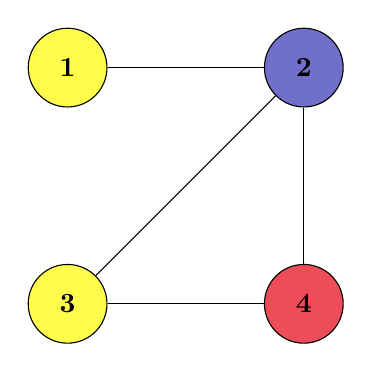
\begin{tikzpicture}[x=1.5cm, y=1.5cm]
  % 設定
  \tikzset{node/.style={circle,draw=black,minimum size=1cm}}
 
  %色
  \definecolor{red}{RGB}{230,0,18}
  \definecolor{blue}{RGB}{51,51,179}
  \definecolor{yellow}{RGB}{255,251,0}
  \definecolor{green}{RGB}{0,96,0}
 
  % 補助線
  % \draw [help lines,blue] (0,0) grid (20,6);
 
  % node %
  \node[node, fill=yellow!70] at (-1,1) (node1) {\textbf{1}};
  \node[node, fill=blue!70] at (1,1) (node2) {\textbf{2}};
  \node[node, fill=yellow!70] at (-1,-1) (node3) {\textbf{3}};
  \node[node, fill=red!70] at (1,-1) (node4) {\textbf{4}};
 
  \foreach \u / \v in {node1/node2, node2/node3, node2/node4, node3/node4}
  \draw (\u) -- (\v);
\end{tikzpicture}
}\\
    && {\Large $\Downarrow$} \\
    \scalebox{0.5}{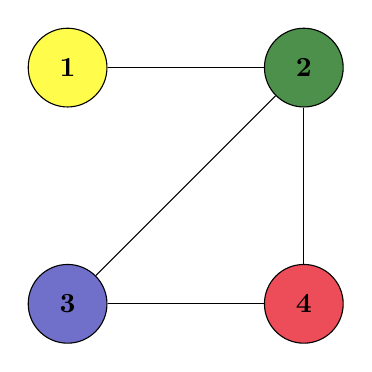
\begin{tikzpicture}[x=1.5cm, y=1.5cm]
  % 設定
  \tikzset{node/.style={circle,draw=black,minimum size=1cm}}
 
  %色
  \definecolor{red}{RGB}{230,0,18}
  \definecolor{blue}{RGB}{51,51,179}
  \definecolor{yellow}{RGB}{255,251,0}
  \definecolor{green}{RGB}{0,96,0}
 
  % 補助線
  % \draw [help lines,blue] (0,0) grid (20,6);
 
  % node %
  \node[node, fill=yellow!70] at (-1,1) (node1) {\textbf{1}};
  \node[node, fill=green!70] at (1,1) (node2) {\textbf{2}};
  \node[node, fill=blue!70] at (-1,-1) (node3) {\textbf{3}};
  \node[node, fill=red!70] at (1,-1) (node4) {\textbf{4}};
 
  \foreach \u / \v in {node1/node2, node2/node3, node2/node4, node3/node4}
  \draw (\u) -- (\v);
\end{tikzpicture}
} &
    \rz{\Large$\Leftarrow$} &
    \scalebox{0.5}{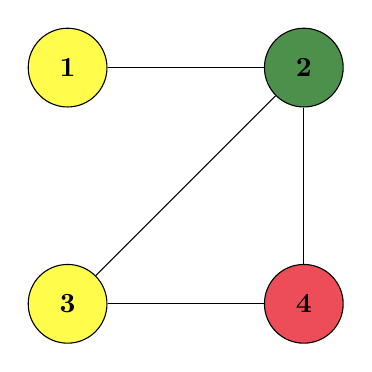
\begin{tikzpicture}[x=1.5cm, y=1.5cm]
  % 設定
  \tikzset{node/.style={circle,draw=black,minimum size=1cm}}
 
  %色
  \definecolor{red}{RGB}{230,0,18}
  \definecolor{blue}{RGB}{51,51,179}
  \definecolor{yellow}{RGB}{255,251,0}
  \definecolor{green}{RGB}{0,96,0}
 
  % 補助線
  % \draw [help lines,blue] (0,0) grid (20,6);
 
  % node %
  \node[node, fill=yellow!70] at (-1,1) (node1) {\textbf{1}};
  \node[node, fill=green!70] at (1,1) (node2) {\textbf{2}};
  \node[node, fill=yellow!70] at (-1,-1) (node3) {\textbf{3}};
  \node[node, fill=red!70] at (1,-1) (node4) {\textbf{4}};
 
  \foreach \u / \v in {node1/node2, node2/node3, node2/node4, node3/node4}
  \draw (\u) -- (\v);
\end{tikzpicture}
}\\
    ゴール状態 ($t=3$) && $t=2$
  \end{tabular}
\end{center}
\end{frame}
%%%%%%%%%%%%%%%%%%%%%%%%%%%%%%%%%%%%%%%%%%%%%%%%%%%%%%%%%%%%%%%%%%%
\begin{frame}\frametitle{実験概要}
  \begin{block}{}\centering
    有界組合せ遷移の有効性を評価するにあたり,以下の実験を行った.
  \end{block}
  \bigskip
  \begin{itemize}
  \item \structure{比較に用いたソルバー}
    \begin{itemize}
    \item 基本ソルバー$\cdots$基本アルゴリズムを実装
    \item 改良ソルバー$\cdots$改良アルゴリズムを実装
    \end{itemize}
  \item \structure{比較に用いたASP符号化}
    \begin{itemize}
    \item \code{changed}符号化
    \item \code{unchanged}符号化
    \end{itemize}
  \item \structure{ベンチマーク問題}: \alert{\bf 独自に作成した$k$彩色遷移問題(計90問)}
    \begin{itemize}
    \item \textit{COLOR04}で公開されているグラフ点彩色問題のグラフ127個のうち,
      彩色数が判明している44個~[Tamura+,'09] を候補とした.
    \item 最終的に,彩色数での実行可能解を全列挙することができたグラフ9個を使用した.
    \end{itemize}
  % \item \structure{ステップ長の上限値}: 基となるグラフ点彩色問題の実行
  %   可能解の総数から1引いた数
    % \begin{itemize}
    % \item グラフmyciel4から作成した問題については,{\clingo}が対応している数
    %   よりも解の総数が大きかったため,
    %   上限値を$2^{31}-1$とした.
    % \end{itemize}
    \item \structure{ASPシステム}: \textit{clingo-5.4.0} \textit{jumpy}
    \item \structure{制限時間}: 3600秒/問
    \item \structure{環境}: Mac OS, 3.2GHz 6コア Intel Core i7,64GB メモリ
    \end{itemize}
\end{frame}
%%%%%%%%%%%%%%%%%%%%%%%%%%%%%%%%%%%%%%%%%%%%%%%%%%%%%%%%%%%%%%%%%%%
\begin{frame}\frametitle{独自に作成した$k$彩色遷移問題}

  \begin{exampleblock}{}
    \centering
    \begin{tabular}{lrrr|r}
  グラフ名 & 頂点数 & 辺数 & 彩色数 & 実行可能解の総数 \\ \hline
  1-FullIns\_3 & 30 & 100 & 4 & 50,693,280 \\ 
  le450\_5a & 450 & 5,714 & 5 & 3,840 \\ 
  le450\_5c & 450 & 9,803 & 5 & 120 \\ 
  le450\_5d & 450 & 9,757 & 5 & 960 \\ 
  myciel3 & 11 & 20 & 4 & 12,480 \\ 
  myciel4 & 23 & 71 & 5 & 2,845,658,400 \\ 
  queen5\_5 & 25 & 160 & 5 & 240 \\  
  queen6\_6 & 36 & 290 & 7 & 100,800 \\ 
  queen7\_7 & 49 & 476 & 7 & 20,160 \\
\end{tabular}
  \end{exampleblock}

  \begin{itemize}
  \item 実行可能解の総数は,最小で120個,最大で約28億個である.
  \item 求められた実行可能解から解をランダムに2つ選びベンチマーク問題を作成し,
        各グラフから10問,計90問を作成した.
  \item 今回の実験では,ステップ長の上限値に,実行可能解の総数から1引
    いた数を使用した.
  \end{itemize}
\end{frame}
%%%%%%%%%%%%%%%%%%%%%%%%%%%%%%%%%%%%%%%%%%%%%%%%%%%%%%%%%%%%%%%%%%%
\begin{frame}\frametitle{実験結果: 解けた問題数}

  \begin{exampleblock}{}
    \centering
    \renewcommand{\arraystretch}{1.2}
    \scalebox{0.9}{\begin{tabular}{l|rr|rr} 
  & \multicolumn{2}{c|}{基本ソルバー} & \multicolumn{2}{c}{改良ソルバー} \\
  & \code{changed} & \code{unchanged} & \code{changed} & \code{unchanged} \\ \hline
  解けた問題数(到達可能) & 11 & 11 & 11 & 11 \\
  解けた問題数(到達不能) & 10 & 10 & 56 & \alert{60} \\\hline
  平均 CPU 時間(秒) & 223.796 & 151.341 & 101.758 & \alert{59.095} \\
\end{tabular}}
  \end{exampleblock}

  \begin{itemize}
  \item 90問中71問について,到達可能性を判定できた.
    \begin{itemize}
    \item 到達可能11問,到達不能60問
    \end{itemize}
  \item 改良ソルバーと\code{unchanged}符号化の組合せが,
    最も多くの問題を解いた.平均CPU時間も最も短い.
%  \item 到達可能であることが判定できた問題のうち,最長のステップ長は17であった.
  \item 到達不能なインスタンスについて,インクリメンタル解法を用いた改
    良ソルバーの優位性が確認できた.
  \end{itemize}
\end{frame}
%%%%%%%%%%%%%%%%%%%%%%%%%%%%%%%%%%%%%%%%%%%%%%%%%%%%%%%%%%%%%%%%%%% 
\begin{frame}\frametitle{実験結果: カクタスプロット}

  \begin{figure}[h]
    \centering
    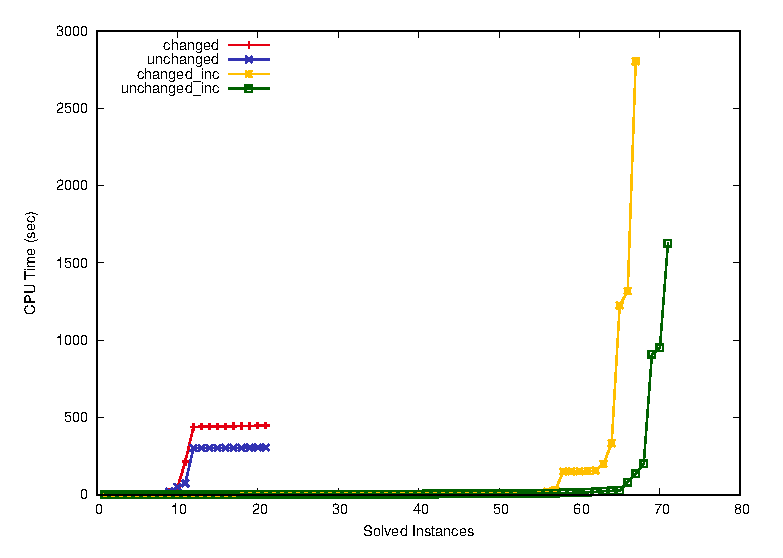
\includegraphics[scale=0.7]{fig/cactus.eps}
  \end{figure}

  \begin{itemize}
    \item 改良ソルバーは基本ソルバーより多くの問題を高速に解いている.
    \item \code{unchanged} 符号化は,\code{changed}符号化より良い性能
      を示した.
  \end{itemize}
  
\end{frame}
%%%%%%%%%%%%%%%%%%%%%%%%%%%%%%%%%%%%%%%%%%%%%%%%%%%%%%%%%%%%%%%%%%%
\begin{frame}\frametitle{まとめ}

  \begin{alertblock}{本研究の貢献}\centering
    ASP を用いた組合せ遷移問題の解法として有界組合せ遷移を提案し,
    汎用ソルバーの実装および$k$彩色遷移問題を用いた性能評価を行なった.
  \end{alertblock}

  \begin{enumerate}
  \item \structure{2種類の実装方式の考案}
    \begin{itemize}
    \item 基本アルゴリズム
    \item インクリメンタルASP解法を用いた改良アルゴリズム
    \end{itemize}
  \item \structure{$k$彩色遷移問題を解く2種類の ASP 符号化の考案}
    \begin{itemize}
    \item $k$彩色遷移問題を簡潔に記述できることを確認
    \end{itemize}
  \item \structure{$k$彩色遷移問題のベンチマーク問題を独自に生成}
  \item \structure{$k$彩色遷移問題を用いた有界組合せ遷移の評価実験}
    \begin{itemize}
    \item 改良アルゴリズムの優位性を確認
    \end{itemize}
  \end{enumerate}
  
  \begin{exampleblock}{今後の課題}
    \begin{itemize}
      \item ソルバーの高速化,組合せ遷移問題の記述例の蓄積
      \item $k$彩色遷移問題の ASP 符号化の改良
    \end{itemize}
  \end{exampleblock}
\end{frame}
%%%%%%%%%%%%%%%%%%%%%%%%%%%%%%%%%%%%%%%%%%%%%%%%%%%%%%%%%%%%%%%%%%%
%\end{document}
%%%% 補助スライド

\begin{frame}{~}
 \centering
 - 補足用 -
\end{frame} 

\begin{frame}{補足 : スマートグリッド}
 \begin{itemize}
  \item \structure{スマートグリッド}とは,電力の供給側,需要側において双方向の
		やり取りを可能にする次世代の\structure{賢い}電力網である.
  \item 従来と違い,通信技術の発達により,使用状況などを
		リアルタイムに把握することが可能となった.
  \item その時に応じた最適な配電網を構成し,制御するといったことが考えられている.
		\begin{itemize}
		 \item 電力需要の変化による,配電ロスの少ない構成.
		 \item 自然エネルギーによる発電量の変動を補う構成.
		\end{itemize}
  \item ASP言語の表現力や拡張性が,こうした条件の追加に活用できる可能性がある.
 \end{itemize}
\end{frame}

%%%%%%%%%%%%%%%%%%%%%%%%%%%%%%%%%%%%%%%%%%%%%%%%%%
%% 電気制約
%%%%%%%%%%%%%%%%%%%%%%%%%%%%%%%%%%%%%%%%%%%%%%%%%%
\begin{frame}{補足 : 電気制約}
 \begin{itemize}
  \item \alert{電気制約}は,送電する電流$\cdot$電圧の適正範囲を保証する制約.
  \begin{itemize}
   \item 供給経路の各区間で許容電流を超えない.
   \item 電気抵抗による電圧降下が許容範囲を超えない.
   \item etc.
  \end{itemize}
  \item 電流と電圧が影響し合う\structure{実数ドメイン上の制約}によって表される.
		% \begin{itemize}
		%  		 \item 送電システム上の条件など.
		% \end{itemize}
  \item 実数ドメイン上の制約は,純粋なASPのみで扱うのは\alert{困難}.
		\begin{itemize}
		 \item 緩和問題として,変電所から供給できる家庭の数に上限をつける.
		 \item ASPMT技術により,ASPで得られた解について,
			   背景理論ソルバーと連携して実数ドメイン上の制約を調べる.
		\end{itemize}
 \end{itemize}
\end{frame}


%%%%%%%%%%%%%%%%%%%%%%%%%%%%%%%%%%%%%%%%%%%%%%%%%%
%% 基礎化
%%%%%%%%%%%%%%%%%%%%%%%%%%%%%%%%%%%%%%%%%%%%%%%%%%
\begin{frame}{補足 : ASPシステム}
 
 \vspace{-0.5cm}

 \begin{figure}[htbp]
  \centering
  %%%%%%%%%%%%%%%%%%%%%%%%%%%%%%%%%%%%%%%%%%%%%%%%%%
%% 基礎化の流れの図
%%%%%%%%%%%%%%%%%%%%%%%%%%%%%%%%%%%%%%%%%%%%%%%%%%
\begin{tikzpicture}

 \definecolor{edge}{RGB}{38,38,134}
 \definecolor{node}{RGB}{220,220,249}

 \definecolor{alert_edge}{RGB}{191,0,0}
 \definecolor{alert_node}{RGB}{249,200,200}

 \definecolor{ex_edge}{RGB}{0,96,0}
 \definecolor{ex_node}{RGB}{230,239,230}

 \def\nodespace{2.4cm}

 \tikzset{block/.style={rectangle, thick, draw=edge, fill=node, text width=3cm, 
 text centered, rounded corners, text width=2cm, minimum height=1.5cm}};

 \tikzset{alertblock/.style={rectangle, thick, draw=alert_edge, fill=alert_node, 
 text width=3cm, text centered, rounded corners, text width=1.5cm, minimum height=1.2cm}};

 \node[block](ikkai){一階ASP\\プログラム};

 \node[rectangle,rounded corners, thick, draw=ex_edge, fill=ex_node, 
 right=0.22*\nodespace of ikkai, minimum width=6cm, minimum height=3cm, 
 text centered, label=ASPシステム](sys){};

 \node[block, right=\nodespace of ikkai](meidai){命題ASP\\プログラム};
 \node[block, right=\nodespace of meidai](ASP){解集合};

 \node[right=0.6*\nodespace of ikkai, text width=1.5cm, 
 text centered, text=red, anchor=south](){基礎化\\ソルバー};
 \node[right=0.4*\nodespace of meidai, text width=1.5cm, 
 text centered, text=red, anchor=south](){解集合\\ソルバー};

 
 \foreach \u / \v / \n in {ikkai/meidai,meidai/ASP}
 \draw [thick,->] (\u) to (\v);

\end{tikzpicture}
 \end{figure}

 \vspace{-0.5cm}

 \begin{exampleblock}{}
  \begin{enumerate}
   \item 一階ASPプログラムを基礎化ソルバーによって,
		 命題ASPプログラムに\alert{基礎化}する.
   \item 命題ASPプログラムについて,SAT技術を応用した解集合ソルバーが解集合を探索する.
  \end{enumerate}
 \end{exampleblock}

\end{frame}


%%%%%%%%%%%%%%%%%%%%%%%%%%%%%%%%%%%%%%%%%%%%%%%%%%
%% ASPのコード
%%%%%%%%%%%%%%%%%%%%%%%%%%%%%%%%%%%%%%%%%%%%%%%%%%
\begin{frame}[fragile]{補足 : 基本符号化のASPプログラム}
 \begin{exampleblock}{}
  \begin{center}
   %%%%%%%%%%%%%%%%%%%%%%%%%%%%%%%%%
   \lstinputlisting[numbers=left,%
   basicstyle=\ttfamily\tiny]{code/srf1.lp}
   %%%%%%%%%%%%%%%%%%%%%%%%%%%%%%%%% 
  \end{center}
 \end{exampleblock}
\end{frame}

\begin{frame}[fragile]{補足 : 改良符号化のASPプログラム}

 \begin{exampleblock}{}
  \begin{center}
   %%%%%%%%%%%%%%%%%%%%%%%%%%%%%%%%%
   \lstinputlisting[numbers=left,%
   basicstyle=\ttfamily\tiny]{code/srf2.lp}
   %%%%%%%%%%%%%%%%%%%%%%%%%%%%%%%%% 
  \end{center}
 \end{exampleblock}

\end{frame}


\end{document}

%%% Local Variables:
%%% mode: japanese-latex
%%% TeX-master: t
%%% End:
